\documentclass[a4paper, 12pt]{article}
\usepackage{graphicx}
\usepackage{float}
\usepackage{listings}
\usepackage[UTF8]{ctex}
\usepackage{xcolor}
\setlength{\parindent}{2em}
\lstdefinestyle{mybash}{
    language=bash,                 % 设置语言为 Bash[reference:8]
    basicstyle=\small\ttfamily,    % 基础字体：使用等宽字体[reference:9][reference:10]
    keywordstyle=\color{blue},     % 关键字颜色[reference:11][reference:12]
    keywordstyle={[2]\color{cyan}},% 第二组关键字颜色[reference:13]
    commentstyle=\itshape\color{orange!70!black}, % 注释样式：斜体 + 橙色[reference:14]
    stringstyle=\color{teal},      % 字符串颜色[reference:15]
    backgroundcolor=\color{yellow!10}, % 背景色：浅黄色[reference:16][reference:17]
    frame=single,                  % 代码框样式[reference:18]
    numbers=left,                  % 在左侧显示行号[reference:19]
    numberstyle=\tiny\color{gray}, % 行号样式[reference:20]
    breaklines=true,               % 自动换行
    showstringspaces=false,        % 不显示字符串中的空格[reference:21][reference:22]
}
\lstdefinestyle{plaintext}{
    language={},                    % 设置语言为空
    basicstyle=\small\ttfamily,    % 基础字体：使用等宽字体
    stringstyle=\color{teal},      % 字符串颜色
    backgroundcolor=\color{yellow!10}, % 背景色：浅黄色[reference:16][reference:17]
    frame=single,                  % 代码框样式
    numbers=left,                  % 在左侧显示行号
    numberstyle=\tiny\color{gray}, % 行号样式
    breaklines=true,               % 自动换行
    showstringspaces=false,        % 不显示字符串中的空格
}
\begin{document}
  \title{Week02 实验报告}
  \author{mrw1114}
  \date{August, 31st}
  \maketitle
  \section{个人信息}
  \begin{itemize}
    \item 姓名：王俊杰
    \item 学号：25020007122
    \item Github 仓库链接：https://github.com/mrw1114/fundamentals-of-system-dev-tools
  \end{itemize}
  \section{课上实验}
    \subsection{第05题：控制一个可清理的后台任务}
      \subsubsection{保存脚本，赋予权限，并在前台启动}
      将内容保存到 worker.sh，用 chmod 赋予可执行权限，启动脚本并把输出流和错误流分别重定向到 stdout.log 和 stderr.log。
      \noindent
      \begin{figure}[H]
        \centering
        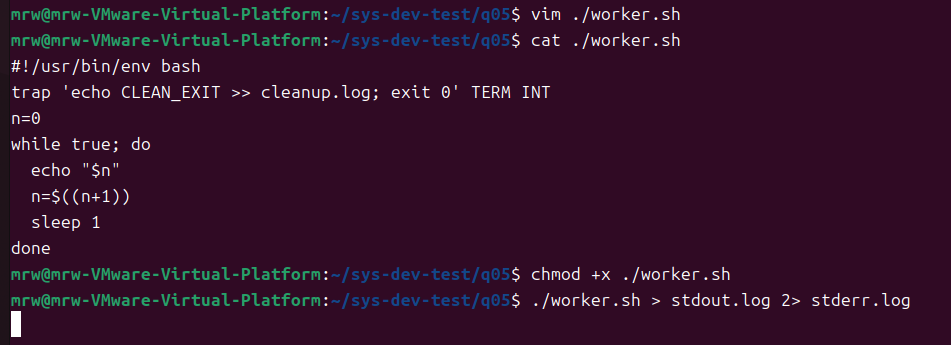
\includegraphics[width=\textwidth]{./05-1.png}
        \caption{运行与重定向}
        \label{05-1}
      \end{figure}
      \subsubsection{挂起程序并转到后台运行}
      使用 Ctrl + Z 将正在运行的进程挂起，再使用 bg 将其置于后台运行，用 jobs 确认其状态。
      \noindent
      \begin{figure}[H]
        \centering
        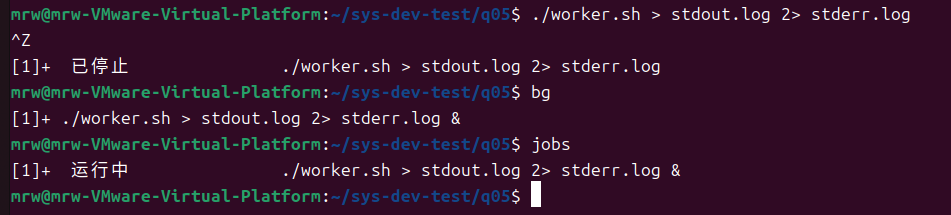
\includegraphics[width=\textwidth]{./05-2.png}
        \caption{挂起与后台运行}
        \label{05-2}
      \end{figure}
      \subsubsection{获取 pid 并向其发送 SIGTERM}
      用 jobs -p \%1 获取我们放入后台运行的程序的 pid，利用命令替换特性将其 pid 传入 kill -TREM 中从而向该进程发送 SIGTERM。最后检查 cleanup.log。 
      \noindent
      \begin{figure}[H]
        \centering
        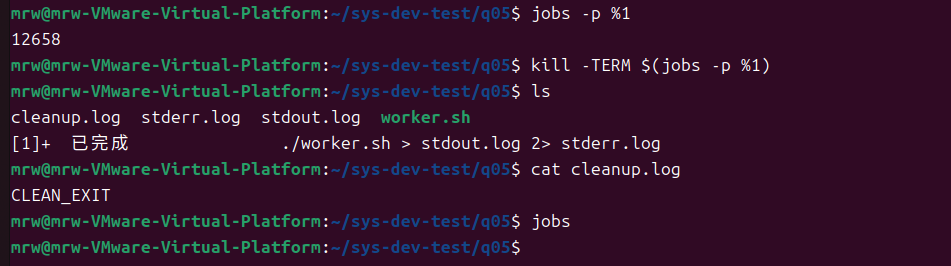
\includegraphics[width=\textwidth]{./05-3.png}
        \caption{运行与重定向}
        \label{05-3}
      \end{figure}
    \subsection{第06题：语义重构与本地开发反馈}
      \noindent
      由于配置问题，本题目在 Windows 环境下使用 VS Code IDE 与 Python 插件、Pylance 语言服务器进行。
      \subsubsection{创建文件}
      新建 q06 文件夹，用 VS Code 打开并新建对应的三个文件。
      \noindent
      \begin{figure}[H]
        \centering
        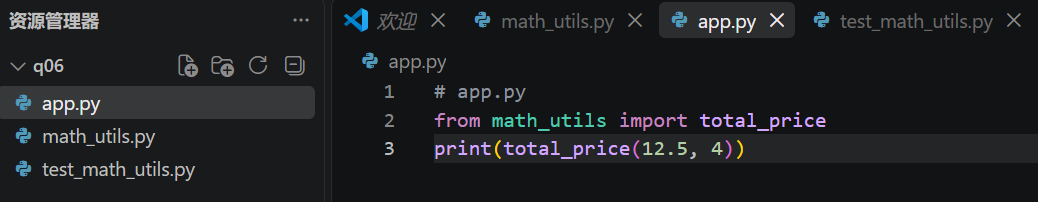
\includegraphics[width=\textwidth]{./06-1-1.png}
        \caption{math\_utils.py 内容}
        \label{06-1-1}
      \end{figure}
      \noindent
      \begin{figure}[H]
        \centering
        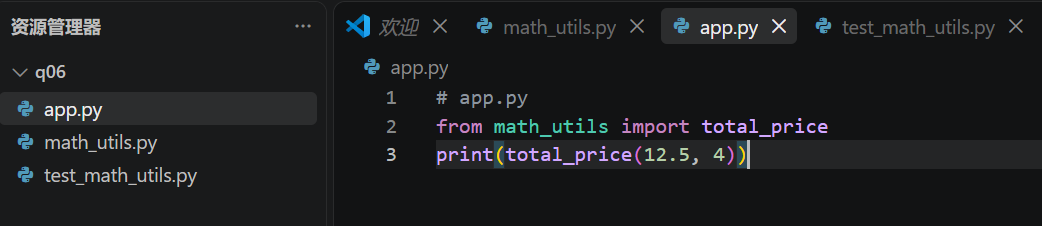
\includegraphics[width=\textwidth]{./06-1-2.png}
        \caption{app.py 内容}
        \label{06-1-2}
      \end{figure}
      \noindent
      \begin{figure}[H]
        \centering
        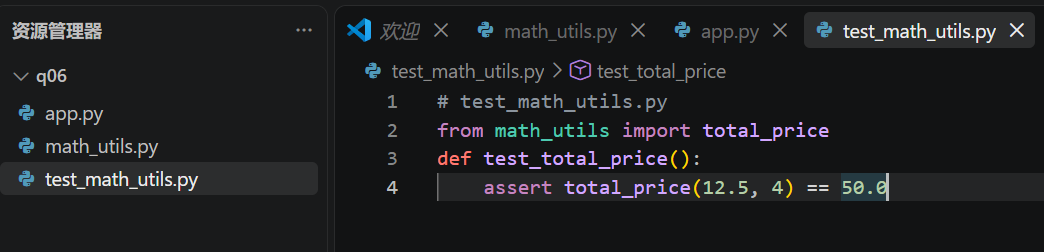
\includegraphics[width=\textwidth]{./06-1-3.png}
        \caption{test\_math\_utils.py 内容}
        \label{06-1-3}
      \end{figure}
      \subsubsection{配置语言服务器并对 total\_price 函数转到定义和查找所有引用}
      打开 VS Code 的设置，修改 Python Language Server 选项为 Pylance。随后打开 app.py，Ctrl + Click 即可转到其在 math\_utils.py 中的定义，右键菜单可点击查找所有引用显示其引用。
      \noindent
      \begin{figure}[H]
        \centering
        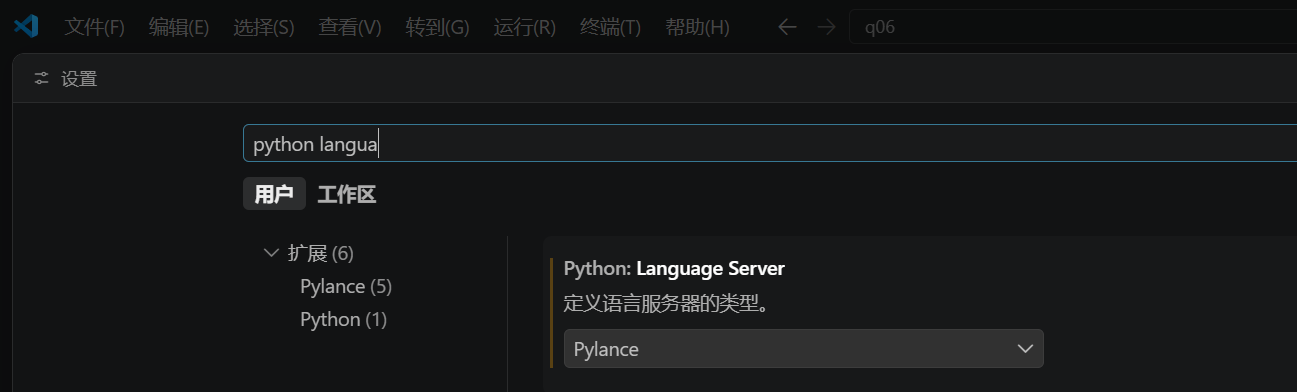
\includegraphics[width=\textwidth]{./06-2-1.png}
        \caption{配置语言服务器}
        \label{06-2-1}
      \end{figure}
      \noindent
      \begin{figure}[H]
        \centering
        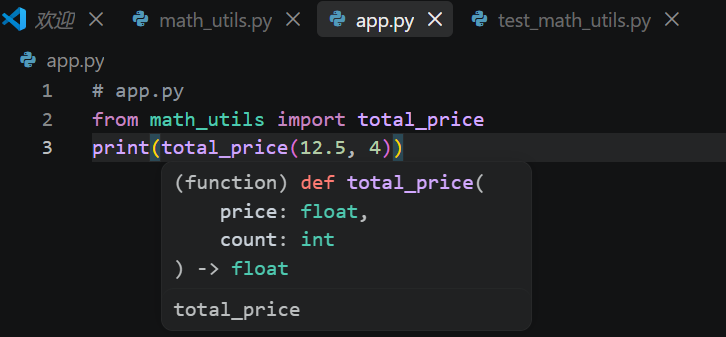
\includegraphics[width=\textwidth]{./06-2-2.png}
        \caption{转到 total\_price 定义}
        \label{06-2-2}
      \end{figure}
      \noindent
      \begin{figure}[H]
        \centering
        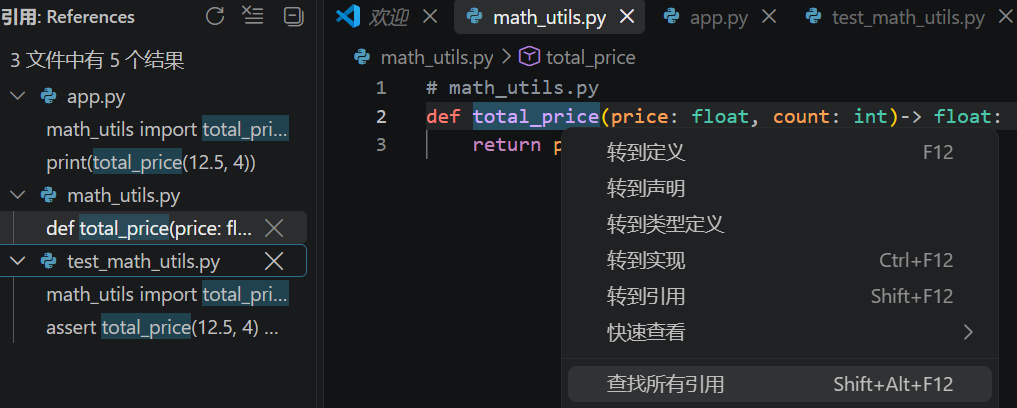
\includegraphics[width=\textwidth]{./06-2-3.png}
        \caption{查找 total\_price 所有引用}
        \label{06-2-3}
      \end{figure}
      \subsubsection{重命名符号}
      右键 total\_price 并选择重命名符号，将其命名为 calculate\_total。
      \noindent
      \begin{figure}[H]
        \centering
        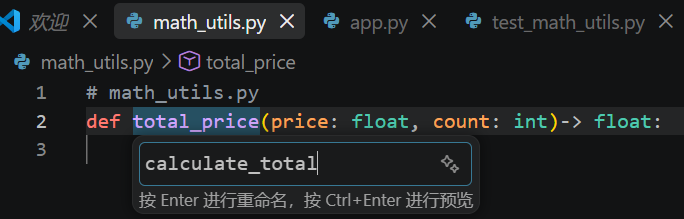
\includegraphics[width=\textwidth]{./06-3.png}
        \caption{重命名符号}
        \label{06-3}
      \end{figure}
      \subsubsection{创建文件}
      向 app.py 中添加未使用的 import os，随后终端运行 ruff check . 检查当前目录下的问题，发现2处格式问题和1处未使用的 import 。通过 ruff check . \detokenize{--}fix 将三处问题修复。随后 pytest 检查通过
      \noindent
      \begin{figure}[H]
        \centering
        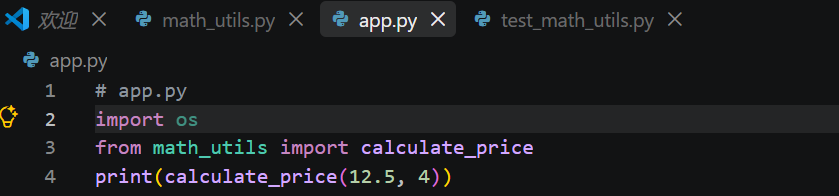
\includegraphics[width=\textwidth]{./06-4-1.png}
        \caption{写入未使用的 imort os}
        \label{06-4-1}
      \end{figure}
      \noindent
      \begin{figure}[H]
        \centering
        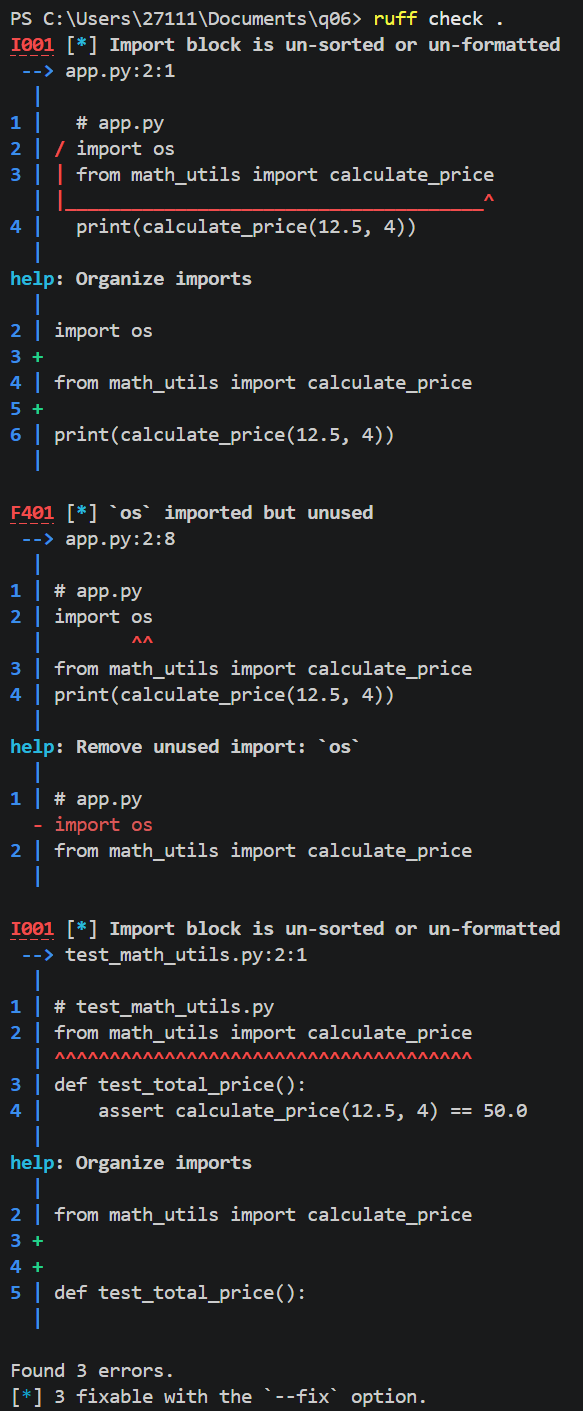
\includegraphics[width=\textwidth]{./06-4-2.png}
        \caption{ruff 检查结果}
        \label{06-4-2}
      \end{figure}
      \noindent
      \begin{figure}[H]
        \centering
        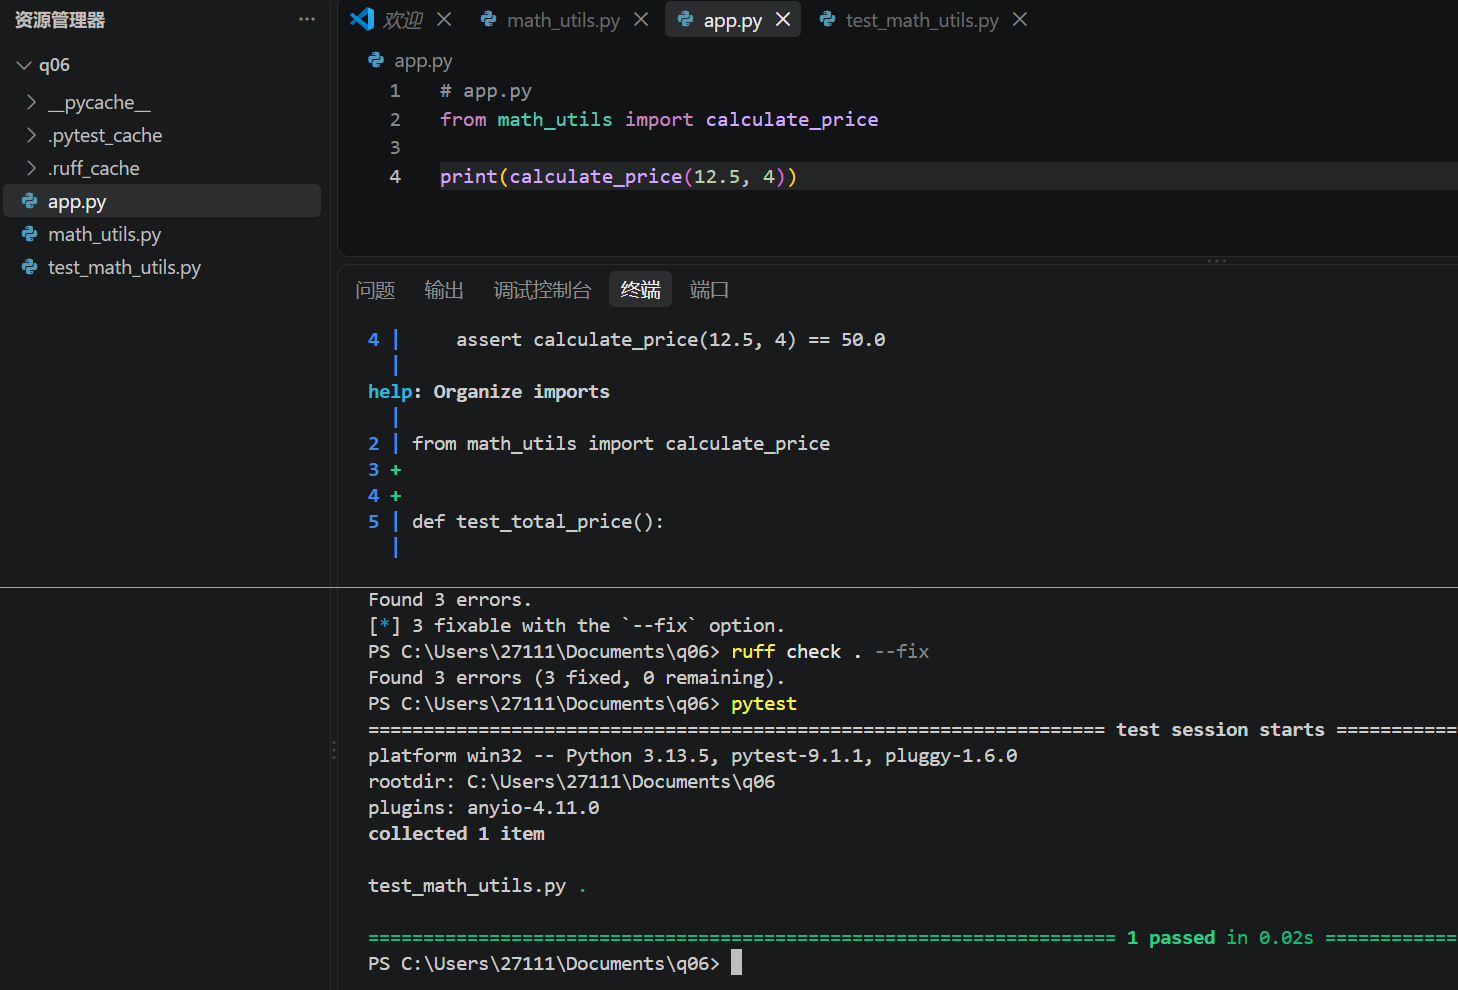
\includegraphics[width=\textwidth]{./06-4-3.png}
        \caption{ruff 修复与 pytest 结果}
        \label{06-4-3}
      \end{figure}
    \subsection{第07题：用调试器定位归并排序缺陷}
      建立虚拟环境如下，安装 ruff 和 pytest，随后启用虚拟环境。
      \noindent
      \begin{figure}[H]
        \centering
        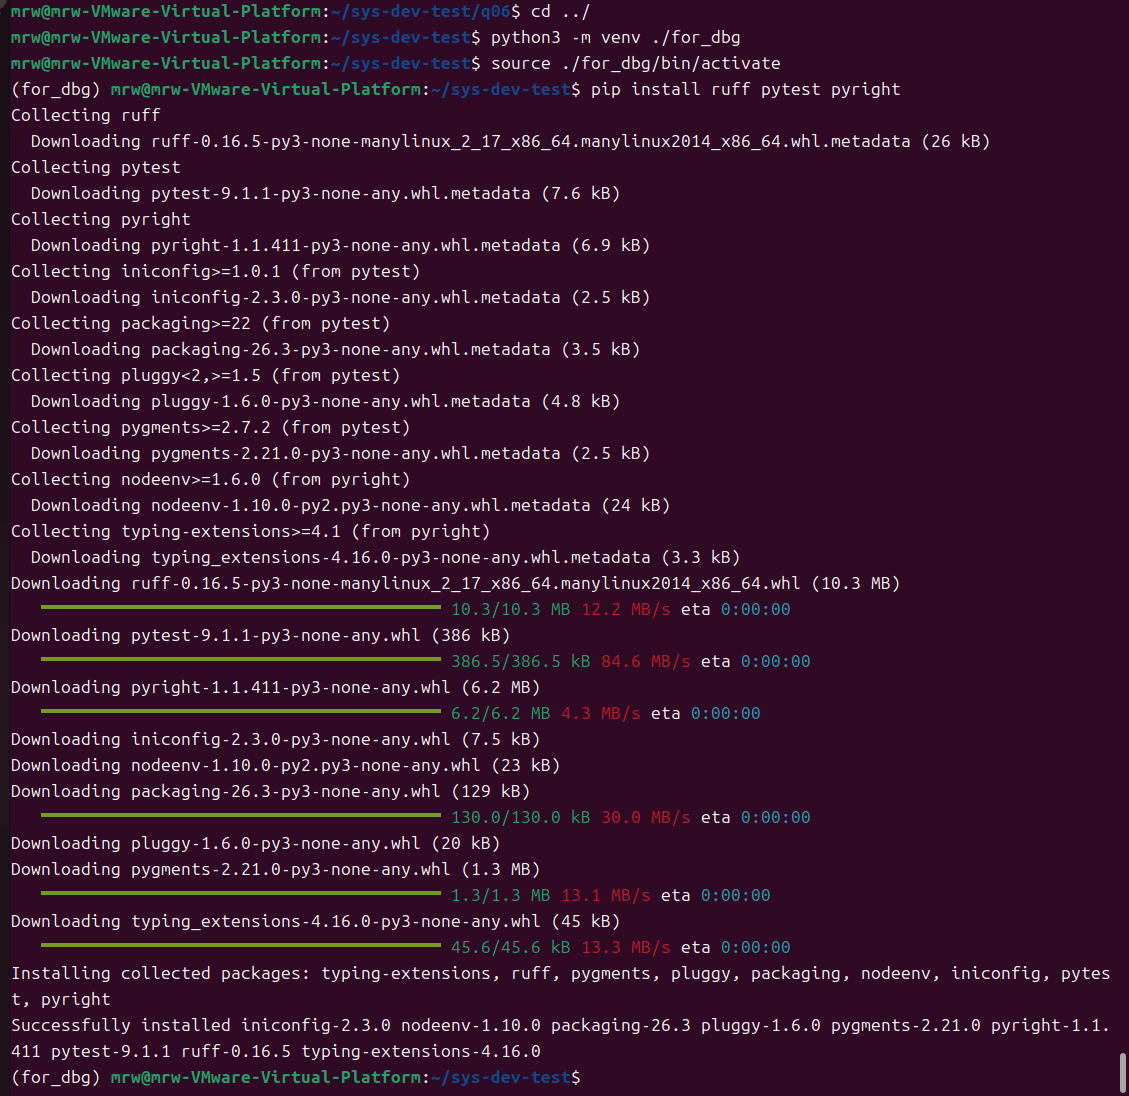
\includegraphics[width=\textwidth]{./environment.png}
        \caption{配置环境}
        \label{env-set}
      \end{figure}
      \subsubsection{创建有问题的归并排序代码文件并观察其输出}
      将有缺陷的代码写入 merge\_sort.py 中，运行查看其输出结果。
      \noindent
      \begin{figure}[H]
        \centering
        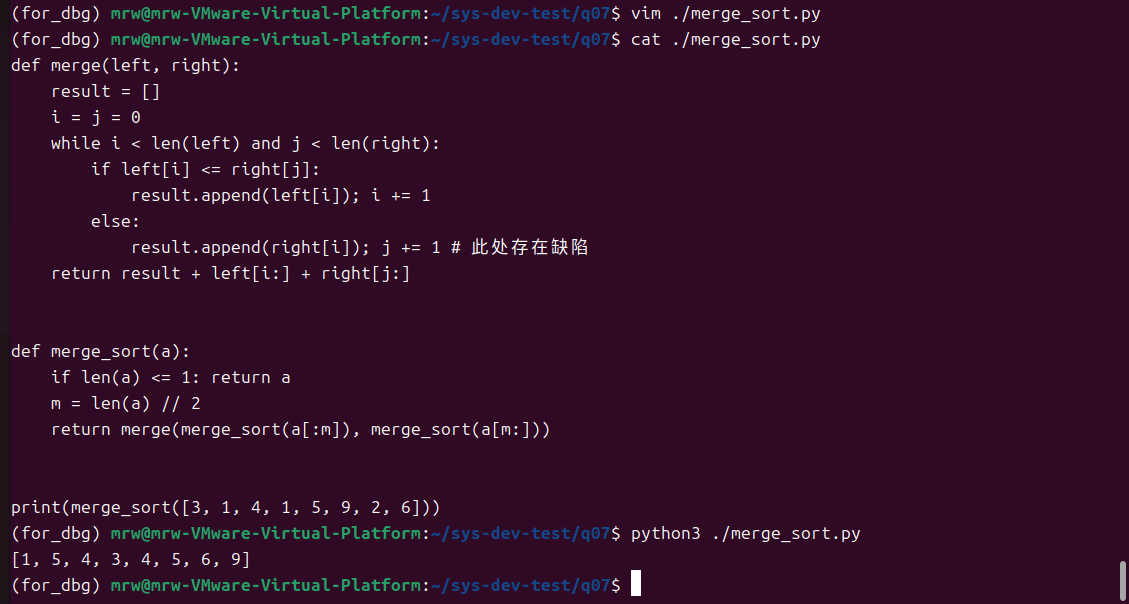
\includegraphics[width=\textwidth]{07-1.png}
        \caption{有缺陷的代码及其输出结果}
        \label{07-1}
      \end{figure}
      \subsubsection{用 pdb 进行调试并观察 merge 执行过程中的变量变化}
      使用 python -m pdb ./merge\_sort.py 进入调试器，设置断点以及中断时执行的命令，查看运行过程中 i, j, left[i], right[j] 的变化。
      \noindent
      \begin{figure}[H]
        \centering
        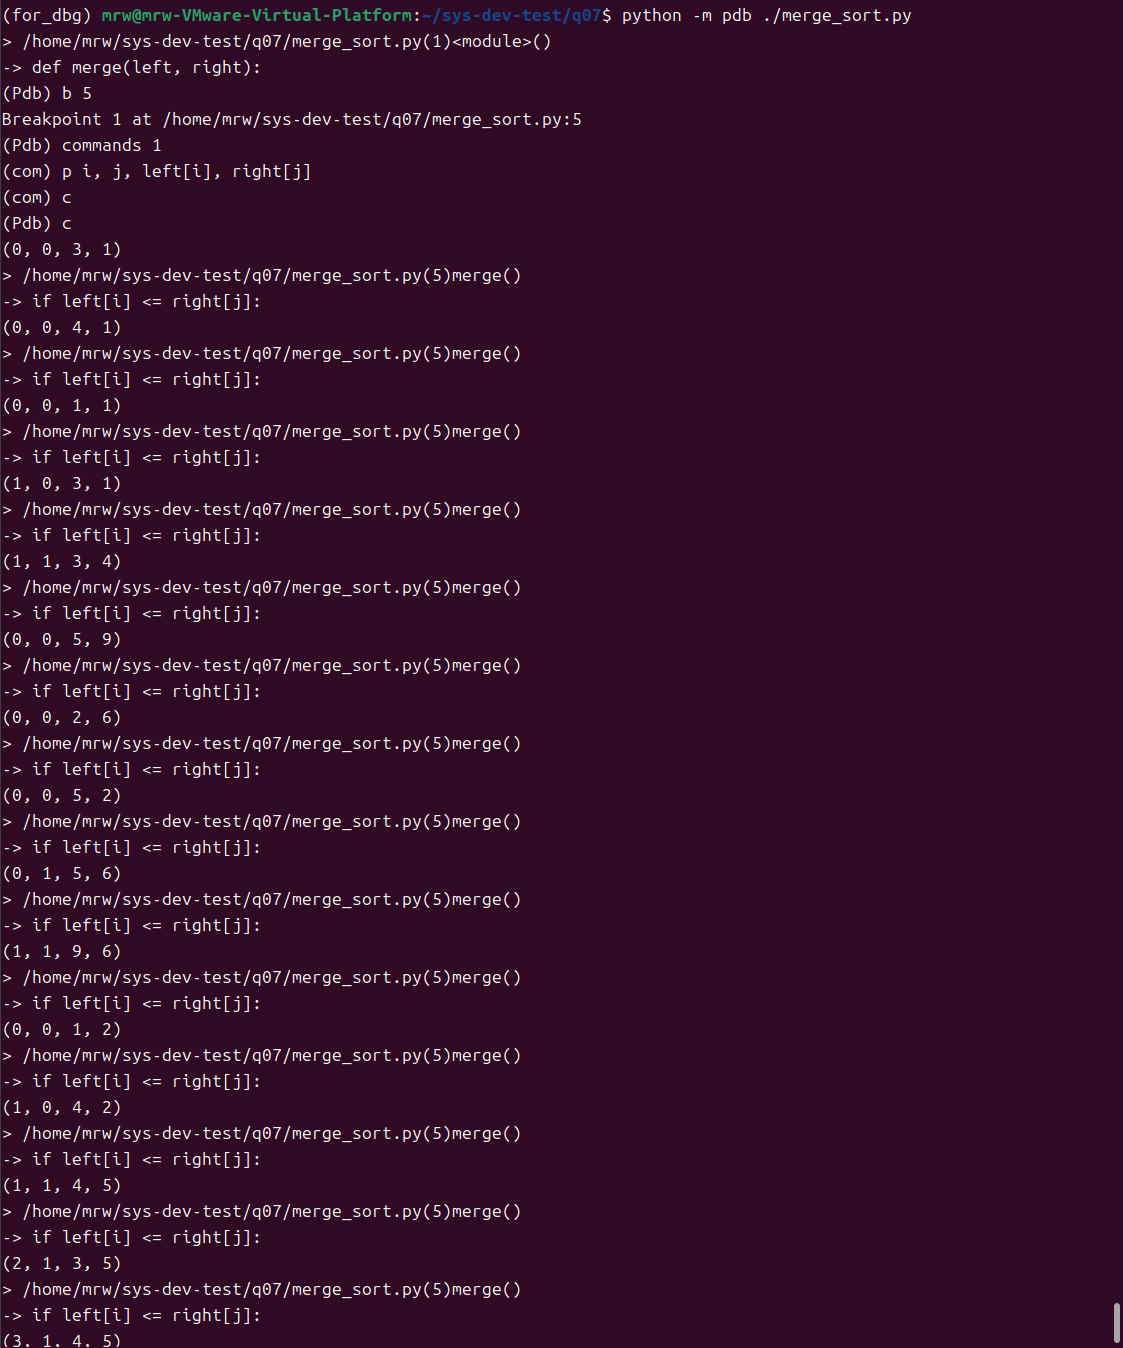
\includegraphics[width=\textwidth]{07-2.png}
        \caption{调试结果}
        \label{07-2}
      \end{figure}
      \subsubsection{修正问题并查看输出结果}
      代码中当 left[i] > right[j] 时应当将 right[j] 置入 result 中，而非 right[i]。修正代码后查看输出结果
      \noindent
      \begin{figure}[H]
        \centering
        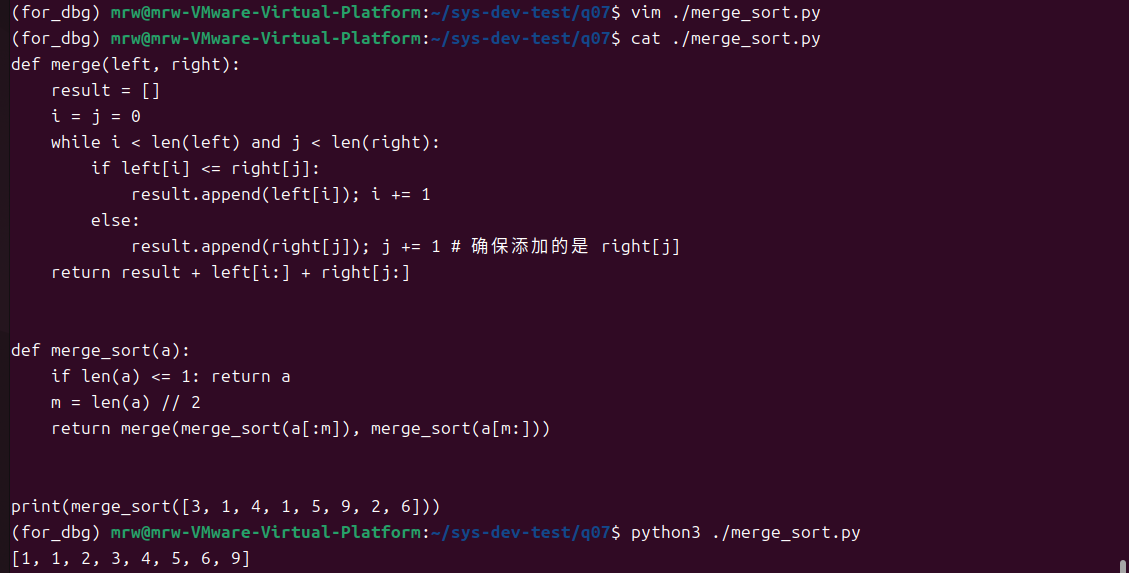
\includegraphics[width=\textwidth]{07-3.png}
        \caption{问题修正后的输出}
        \label{07-3}
      \end{figure}
      \subsubsection{增加测试文件并使用 pytest 检验}
      新建 test\_merge\_sort.py，从 merge\_sort 函数引入 merge\_sort 函数，并定义带有断言的两个测试函数。随后 pytest . 对代码进行测试。
      \noindent
      \begin{figure}[H]
        \centering
        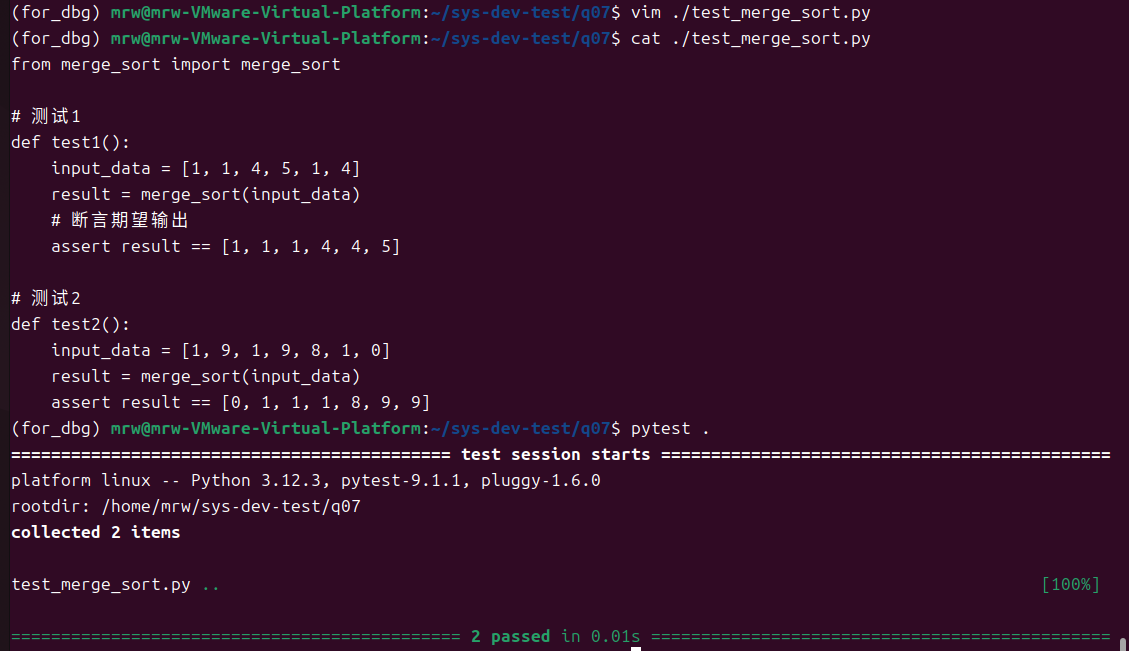
\includegraphics[width=\textwidth]{07-4.png}
        \caption{测试结果}
        \label{07-4}
      \end{figure}
     \subsection{第08题：先测量，再优化慢速词频程序}
      \subsubsection{新建对应文件}
      将对应代码输入对应文件中。
      \noindent
      \begin{figure}[H]
        \centering
        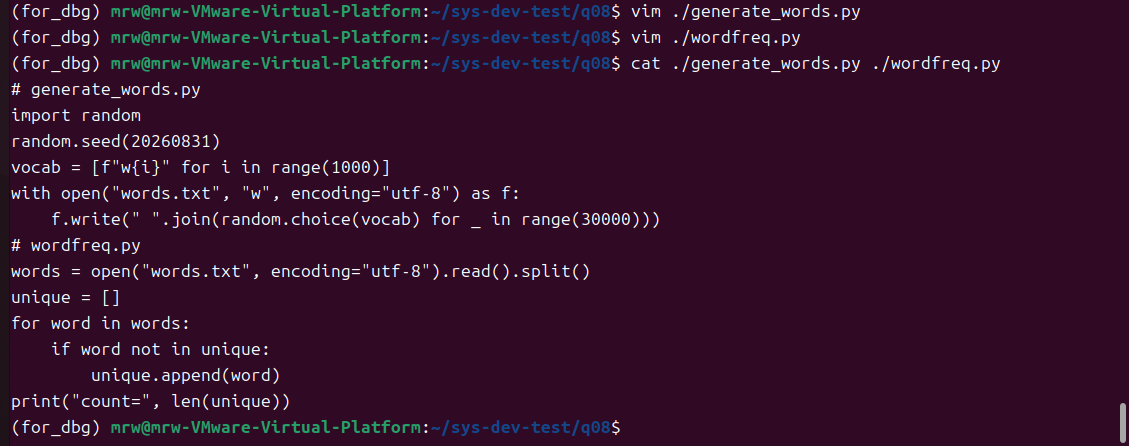
\includegraphics[width=\textwidth]{08-1.png}
        \caption{新建相关文件}
        \label{08-1}
      \end{figure}
      \subsubsection{生成词库，运行原始词频统计程序并记录运行时间}
      运行 generate\_words.py 生成词库 words.txt，随后使用 time 命令运行 ./wordfreq.py 程序两次并记录运行时间。得到一开始的程序运行时间分别为 0.112s 和 0.117s。
      \noindent
      \begin{figure}[H]
        \centering
        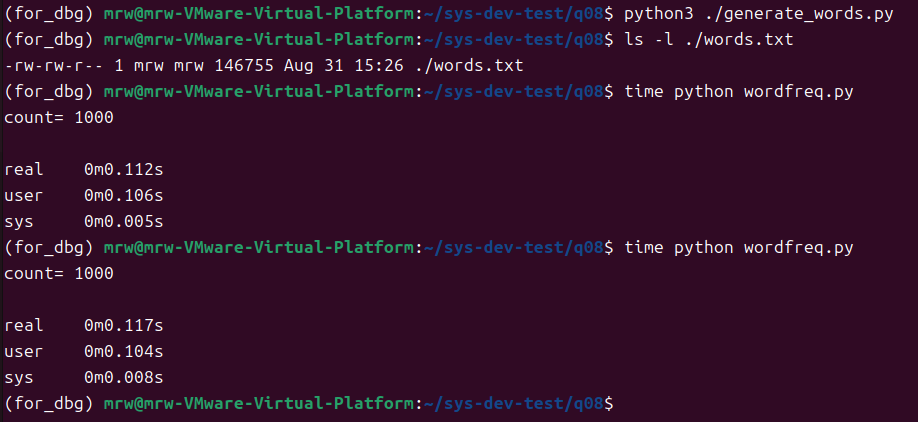
\includegraphics[width=\textwidth]{08-2.png}
        \caption{原始词频统计程序的运行时间}
        \label{08-2}
      \end{figure}
      \subsubsection{分析原始程序主要耗时位置}
      使用 python -m cProfile-s cumulative wordfreq.py 分析耗时分布，发现 split, read 等函数几乎不耗时，append 函数虽然执行 1000 次但总耗时极少，反倒是模块顶层代码耗费了绝大多数的时间。据此分析，应当是因为 if word not in unique 这行判断使用了 in 操作符查找列表内容，而其时间复杂度高达 O(n) 。
      \noindent
      \begin{figure}[H]
        \centering
        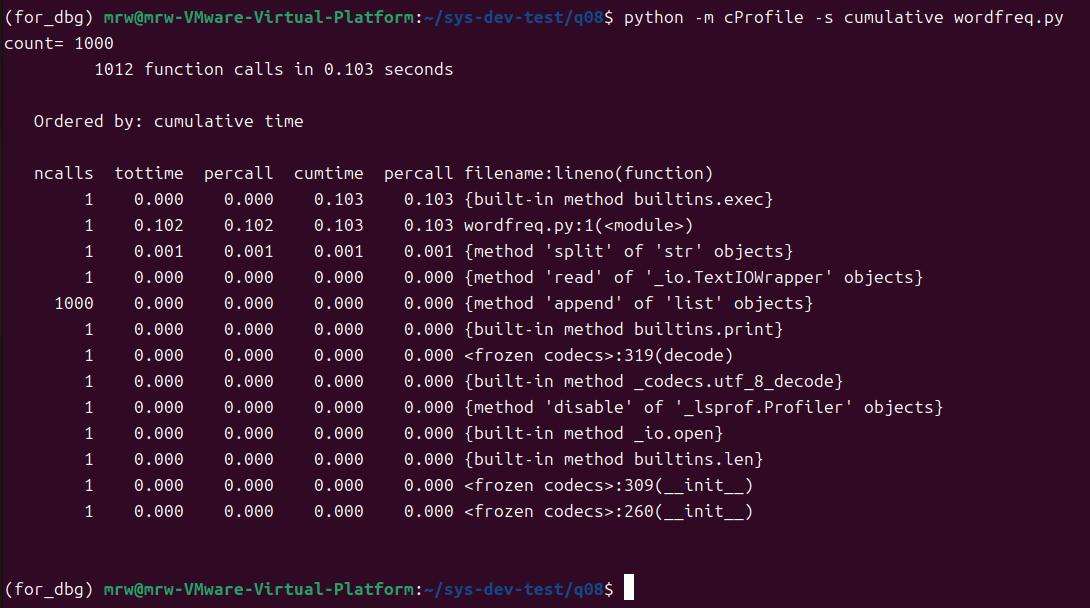
\includegraphics[width=\textwidth]{08-3.png}
        \caption{原始程序耗时分布}
        \label{08-3}
      \end{figure}
      \subsubsection{优化程序并统计优化前后中位数和加速比}
      根据之前的分析，我们可以将 unique 变成集合，这样可以将查询的时间复杂度降到近乎 O(1) ，同时把 append 改为 add。优化后程序运行时间降到 0.014s 和 0.015s 。优化前后程序运行时间中位数分别为 0.1145s 和 0.0145 s，加速比可达 7.897。
      \noindent
      \begin{figure}[H]
        \centering
        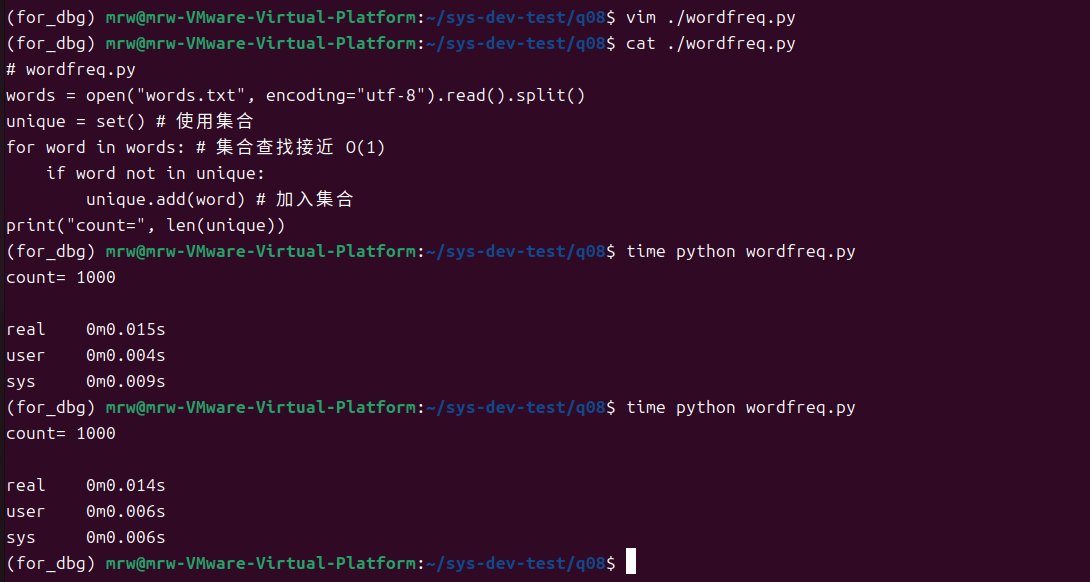
\includegraphics[width=\textwidth]{08-4.png}
        \caption{优化后的程序及其运行时间}
        \label{08-4}
      \end{figure}
  \section{课后练习}
    \subsection{第01题：\detokenize{--}的用途}
      \subsubsection{题目描述}
      你可能见过像 cmd \detokenize{--}flag \detokenize{--} \detokenize{--}notaflag 这样的命令。这里的 \detokenize{--} 是一个特殊参数，它告诉程序后面不要再继续解析选项（flag）了。也就是说，\detokenize{--} 后面的所有内容都会被当作位置参数（positional argument）。这有什么用？试着运行 touch \detokenize{--} -myfile，然后在不使用 \detokenize{--} 的情况下把它删掉。
      \subsubsection{解题过程}
      \detokenize{--} 可以避免将以 - 开头的参数视为选项。想要在不使用 \detokenize{--} 的情况下删除文件名以 - 开头的文件可以通过 rm ./-myfile 。
      \noindent
      \begin{figure}[H]
        \centering
        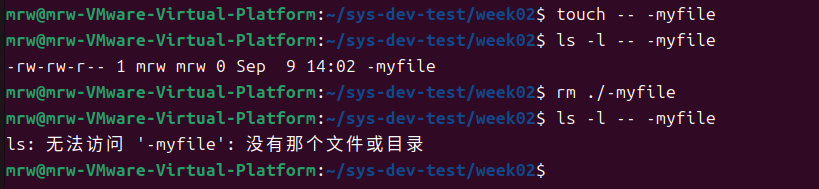
\includegraphics[width=\textwidth]{work02-1.png}
        \caption{-myfile 文件的新建与删除}
        \label{work02-1}
      \end{figure}
    \subsection{第02题：使用 ls 按特定格式列出文件}
      \subsubsection{题目描述}
      阅读 man ls，写出一个 ls 命令，让它按下面的方式列出文件：
      \begin{itemize}
        \item 包含所有文件，包括隐藏文件
        \item 文件大小以易读格式显示（例如 454M，而不是 454279954）
        \item 按最近修改时间排序
        \item 输出带颜色
      \end{itemize}
      \subsubsection{解题过程}
      通过 man ls 进行查阅，可以发现短选项 -a 可以列出包含隐藏文件的所有文件，-l 可以列出文件详细信息，-h 可按人类易读方式列出文件大小，-t 可按文件修改时间从新到旧列出文件，而长选项 \detokenize{--}color 支持带颜色的输出。故可以使用命令 ls -alht \detokenize{--}color 实现题目要求。
      \noindent
      \begin{figure}[H]
        \centering
        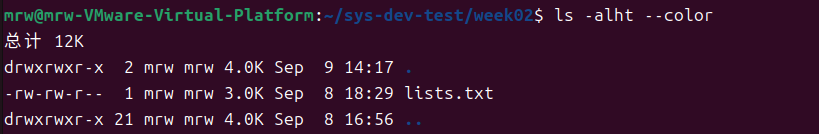
\includegraphics[width=\textwidth]{work02-2.png}
        \caption{使用 ls -alht \detokenize{--}color 后的输出结果}
        \label{work02-2}
      \end{figure}
    \subsection{第03题：printenv 与 export 的差异比较}
      \subsubsection{题目描述}
      进程替换 <(command) 可以让你把一个命令的输出当成文件来用。试着配合 diff 和进程替换，比较 printenv 与 export 的输出。它们为什么不一样？（提示：可以试试 diff <(printenv | sort) <(export | sort)）
      \subsubsection{解题过程}
      printenv 和 export 都会输出 shell 的环境变量（会传递给子进程的变量），区别在于 printenv 仅会输出环境变量键值对，而 export 会输出 shell 属性标记如 declare -x VAR=VALUE。
      \noindent
      \begin{figure}[H]
        \centering
        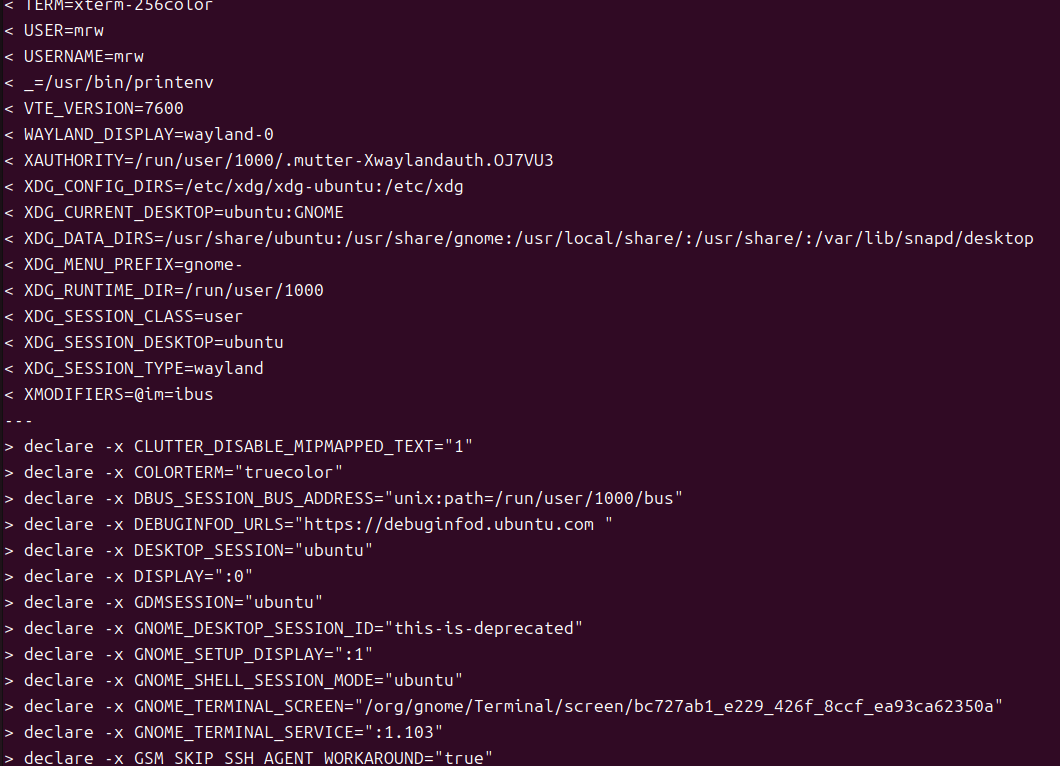
\includegraphics[width=\textwidth]{work02-3.png}
        \caption{命令执行后的部分输出}
        \label{work02-3}
      \end{figure}
    \subsection{第04题：利用 bash 函数与环境变量保存工作目录}
      \subsubsection{题目描述}
      写两个 bash 函数 marco 和 polo，行为如下：每次执行 marco 时，都要以某种方式保存当前工作目录；之后无论你切到哪个目录，只要执行 polo，它都应该把你 cd 回执行 marco 时所在的目录。为了方便调试，你可以把代码写进 marco.sh，然后通过执行 source marco.sh 把这些定义重新加载到当前 shell。
      \subsubsection{解题过程}
      编写 marco 函数使其执行时将 pwd 命令的输出（PWD 变量的值不和工作目录完全绑定）保存到变量 marco\_dir 中，再编写 polo 函数使其执行时通过 cd 命令修改当前目录。据此编写 marco.sh 并通过 source marco.sh 将两个函数加载到 shell 终端里。
\begin{lstlisting}[caption={marco.sh 的内容},style=mybash]
marco() {
    marco_dir=$(pwd)
}
polo() {
    cd $marco_dir || echo "No dir saved."
}
\end{lstlisting}
      \noindent
      \begin{figure}[H]
        \centering
        
\includegraphics[width=\textwidth]{work02-4.png}
        \caption{函数效果演示}
        \label{work02-4}
      \end{figure}
    \subsection{第05题：对产生失败不确定的命令进行调试}
      \subsubsection{题目描述}
      假设你有一个很少失败的命令。为了调试它，你需要把它的输出保存下来，但等到一次失败运行可能会很耗时。写一个 bash 脚本，不断运行下面这个脚本直到它失败为止，并把标准输出和标准错误分别保存到文件里，最后把结果打印出来。如果>你还能顺便报告它运行了多少次才失败，就加分。
\begin{lstlisting}[caption={给定的脚本内容},style=mybash]
#!/usr/bin/env bash

n=$(( RANDOM % 100 ))

if [[ n -eq 42 ]]; then
   echo "Something went wrong"
   >&2 echo "The error was using magic numbers"
   exit 1
fi

echo "Everything went according to plan"
\end{lstlisting}
      \subsubsection{解题过程}
      将给定内容存入 42.sh 脚本，并赋予其可执行权限。随后新建 test 脚本，定义变量 cnt=0 用以记录 42.sh 成功执行次数，将 ./42.sh >> stdout.log 2>> stderr.log 作为 while 语句的执行条件，若语句成功则 while 循环继续执行使计数加1，若执行失败则跳出 while 循环并输出成功执行的次数。
\begin{lstlisting}[caption={test.sh 脚本内容},style=mybash]
#!/bin/bash
cnt=0
while ./42.sh >> stdout.log 2>> stderr.log
do
    cnt=$(($cnt+1))
done

echo "Failed after $cnt runs."
\end{lstlisting}
      \noindent
      \begin{figure}[H]
        \centering
        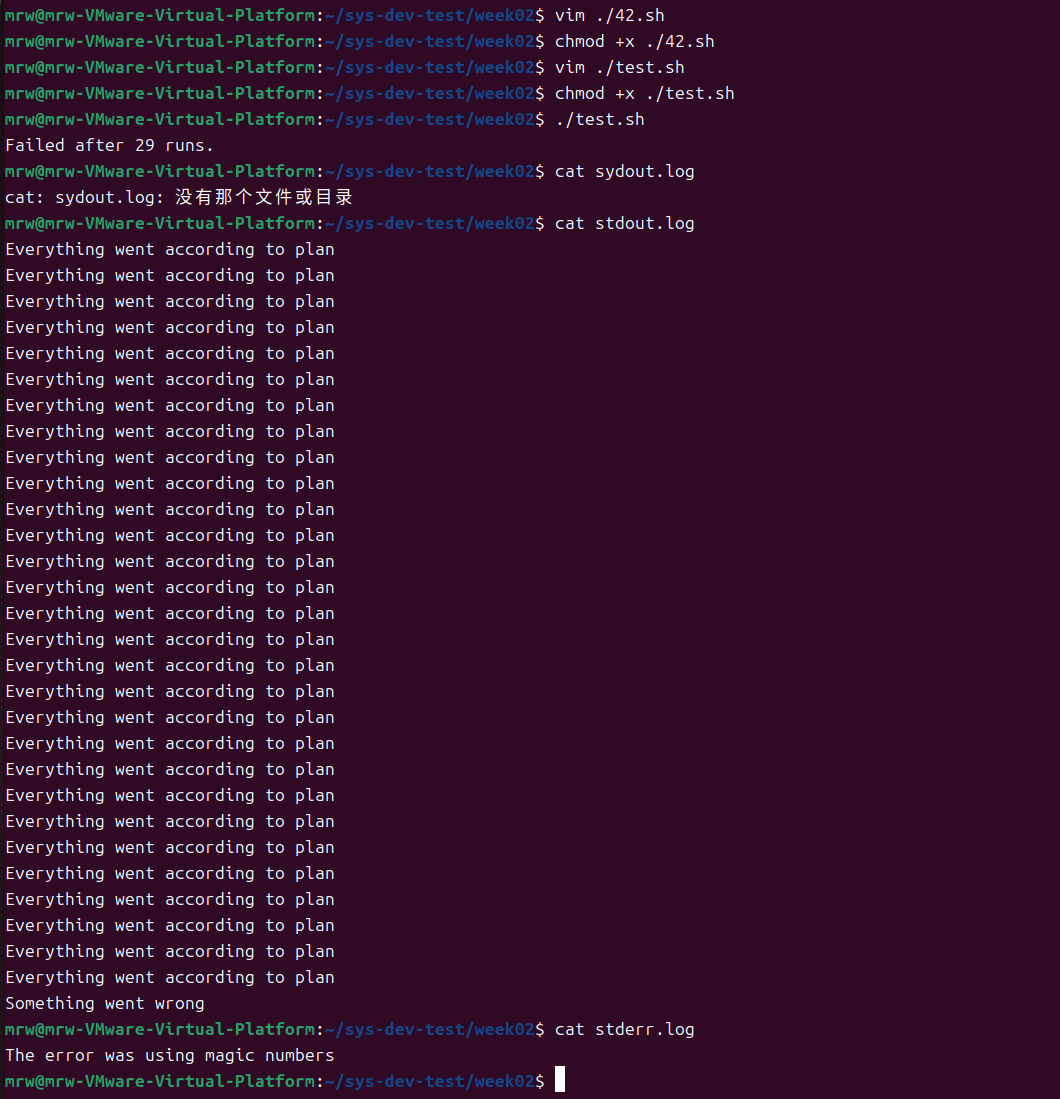
\includegraphics[width=\textwidth]{work02-5.png}
        \caption{test.sh 的执行效果}
        \label{work02-5}
      \end{figure}
    \subsection{第06题：任务管理训练}
      \subsubsection{题目描述}
      在终端里启动一个 sleep 10000 任务，用 Ctrl-Z 把它挂起，再用 bg 让它继续在后台运行。然后使用 pgrep 找到它的 pid，再用 pkill 把它杀掉，整个过程都不要手动输入这个 pid。（提示：试试 -af 参数）
      \subsubsection{解题过程}
      利用 pgrep -af 选项可以根据进程名称查询并展示查找到的 PID 和命令行，利用 pkill -f 可以通过进程名称匹配要结束的进程。
      \noindent
      \begin{figure}[H]
        \centering
        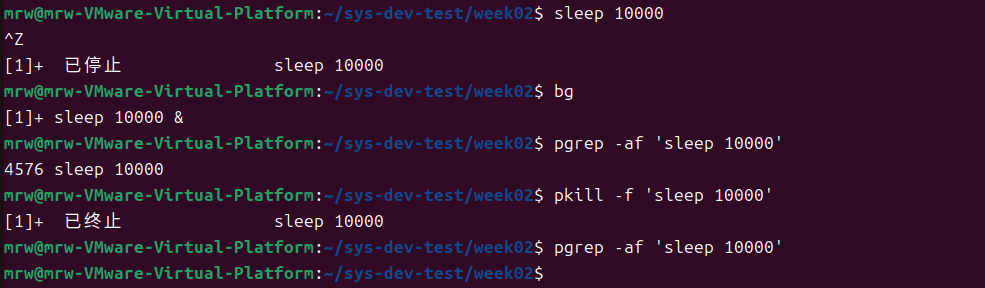
\includegraphics[width=\textwidth]{work02-6.png}
        \caption{进程控制演示结果}
        \label{work02-6}
      \end{figure}
    \subsection{第07题：利用 alias 命令创建 cd 命令的别名}
      \subsubsection{题目描述}
      创建一个 alias dc，让你把 cd 打错时也能正常工作。
      \subsubsection{解题过程}
      使用命令 alias dc="cd" 为 cd 命令创建别名 dc 即可。
      \noindent
      \begin{figure}[H]
        \centering
        
\includegraphics[width=\textwidth]{work02-7.png}
        \caption{cd 别名 dc 的创建与使用效果}
        \label{work02-7}
      \end{figure}
    \subsection{第08题：配置 ssh 密钥}
      \subsubsection{题目描述}
      进入 ~/.ssh/，检查你是否已经有一对 SSH 密钥。如果没有，就用 ssh-keygen -a 100 -t ed25519 生成一对。建议给密钥设置密码，并配合 ssh-agent 使用。
      \subsubsection{解题过程}
      执行 ssh-keygen -a 100 -t ed25519 -f ~/.ssh/id\_ed25519 生成 ssh 密钥并输入使用密钥所需的密码，随后使用 eval "\$(ssh-agent -s)" 启动 ssh 代理进程并向终端注入环境变量，最后用 ssh-add ~/.ssh/id\_ed25519 将生成的 ssh 密钥文件加载到代理中，使得代理运行期间无需再次输入密码验证 ssh 密钥。
      \noindent
      \begin{figure}[H]
        \centering
        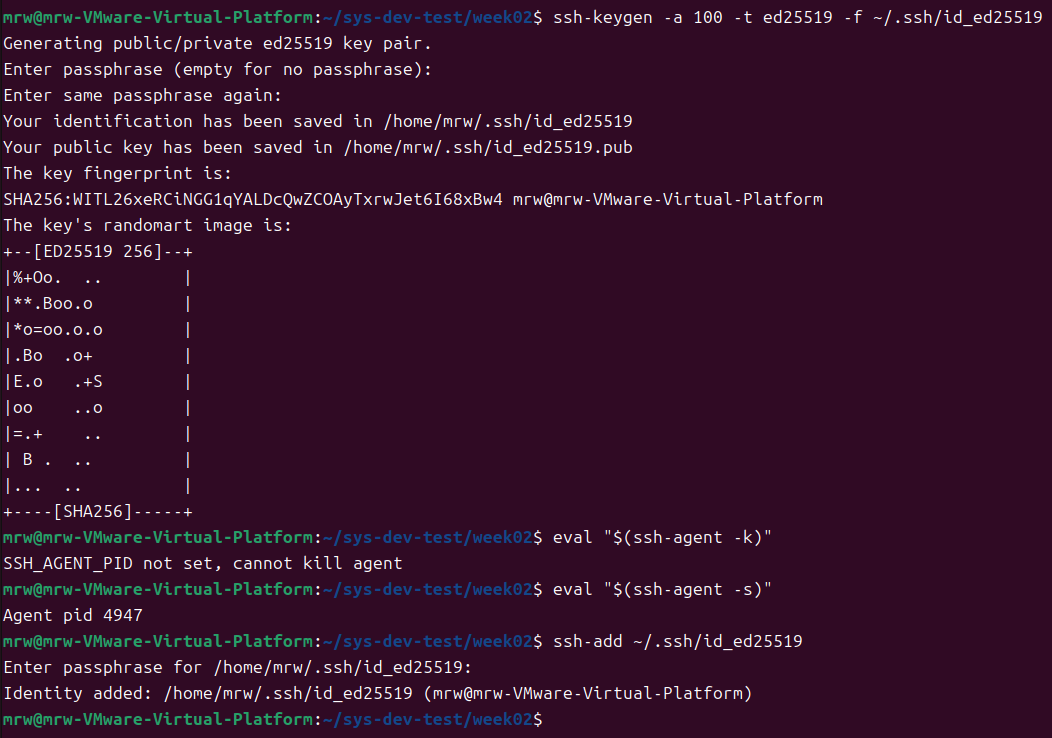
\includegraphics[width=\textwidth]{work02-8.png}
        \caption{ssh 密钥的生成与 ssh-agent 的配置}
        \label{work02-8}
      \end{figure}
    \subsection{第09题：编辑 ssh 配置}
      \subsubsection{题目描述}
      编辑 .ssh/config，加入下面这样的配置项：
\begin{lstlisting}[caption={给定的配置项},style={plaintext}]
Host vm
    User username_goes_here
    HostName ip_goes_here
    IdentityFile ~/.ssh/id_ed25519
    LocalForward 9999 localhost:8888
\end{lstlisting}
      \subsubsection{解题过程}
      通过 ifconfig 获取另一台虚拟机的本地 ip 为 192.168.234.129。用户名为 kali，据此用 vim 填写配置并进行保存。 
      \noindent
      \begin{figure}[H]
        \centering
        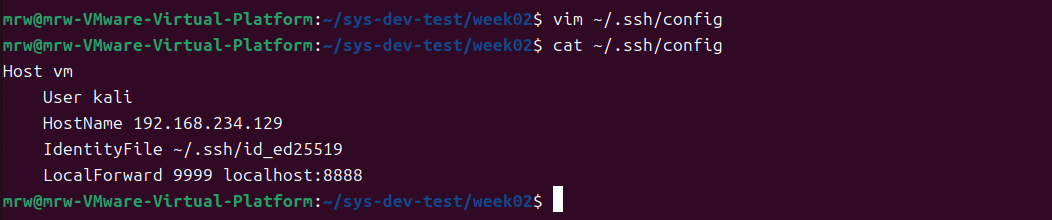
\includegraphics[width=\textwidth]{work02-9.png}
        \caption{编写的 ssh 配置内容}
        \label{work02-9}
      \end{figure}
\subsection{第10题：复制 ssh 公钥到服务器上}
      \subsubsection{题目描述}
      使用 ssh-copy-id vm 把你的 SSH 公钥复制到服务器上。
      \subsubsection{解题过程}
      运行 ssh-copy-id vm 尝试复制 ssh 公钥到服务器上，由于这是第一次连接程序表示主机名称未知，向我们请求是否信任主机，输入 yes 确认连接。随后程序提示我们输入 kali 用户的密码，输入其密码后 ssh 密钥被添加到虚拟机 kali 用户的 authorized\_keys 中。
      \noindent
      \begin{figure}[H]
        \centering
        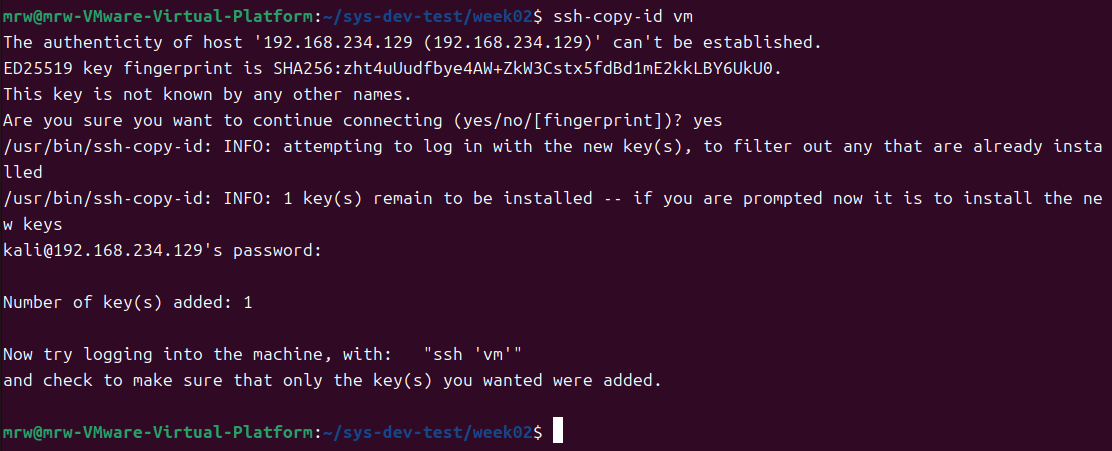
\includegraphics[width=\textwidth]{work02-10.png}
        \caption{使用 ssh-copy-id 将 ssh 密钥复制到虚拟机账户}
        \label{work02-10}
      \end{figure}
\subsection{第11题：启动 Web 服务器并尝试访问}
      \subsubsection{题目描述}
      在虚拟机里执行 python -m http.server 8888 启动一个 Web 服务器。然后在你自己的机器上访问 http://localhost:9999，确认自己能访问虚拟机里的这个服务。
      \subsubsection{解题过程}
      在虚拟机的 kali 账户上执行 python -m http.server 8888 在虚拟机本地的8888端口启动 python 服务器，随后使用 ssh vm 远程登录到虚拟机的 kali 账户。由于 vm 配置中配置了前向转发，在本地的9999端口对应到虚拟机的8888端口，此时在本地访问 http://localhost:9999 即可访问到虚拟机上的 python 服务器。
      \noindent
      \begin{figure}[H]
        \centering
        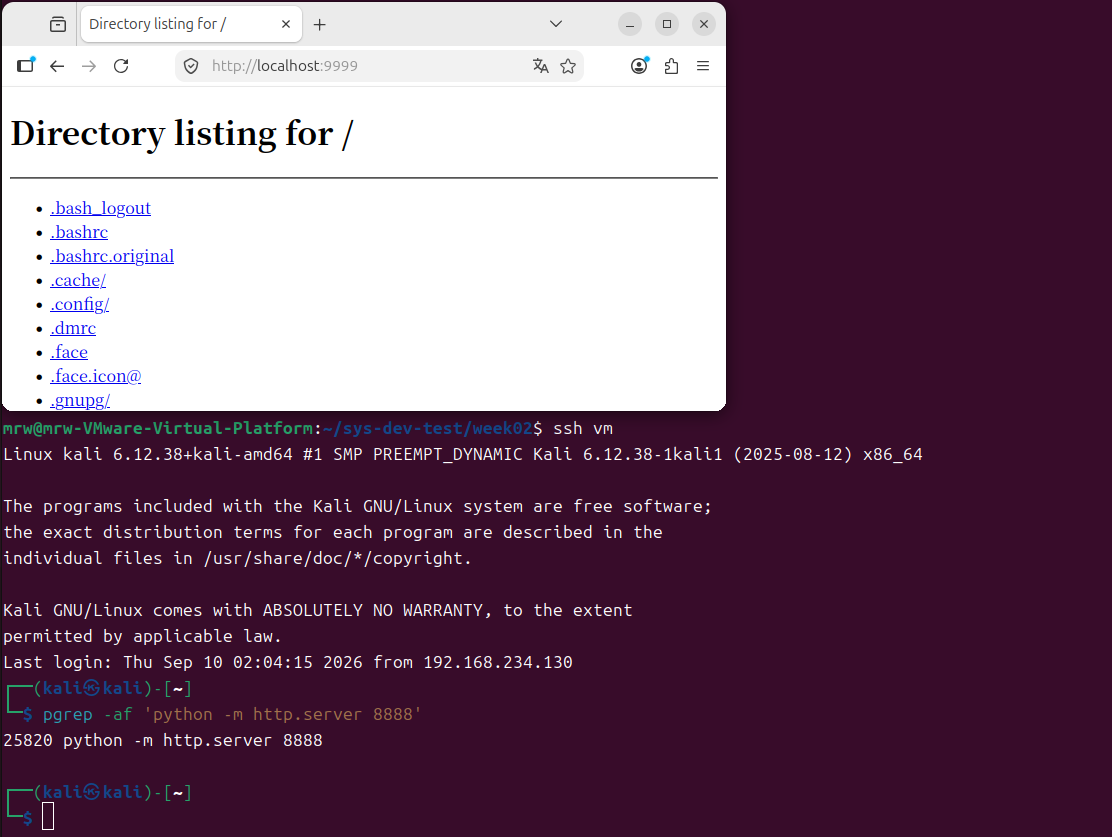
\includegraphics[width=\textwidth]{work02-11.png}
        \caption{利用 ssh 连接到虚拟机并访问 python 服务器}
        \label{work02-11}
      \end{figure}
  \section{commit 记录}
  本周实验所使用的文件的上传记录如下，详细信息请访问 github 仓库。
  \noindent
  \begin{figure}[H]
    \centering
    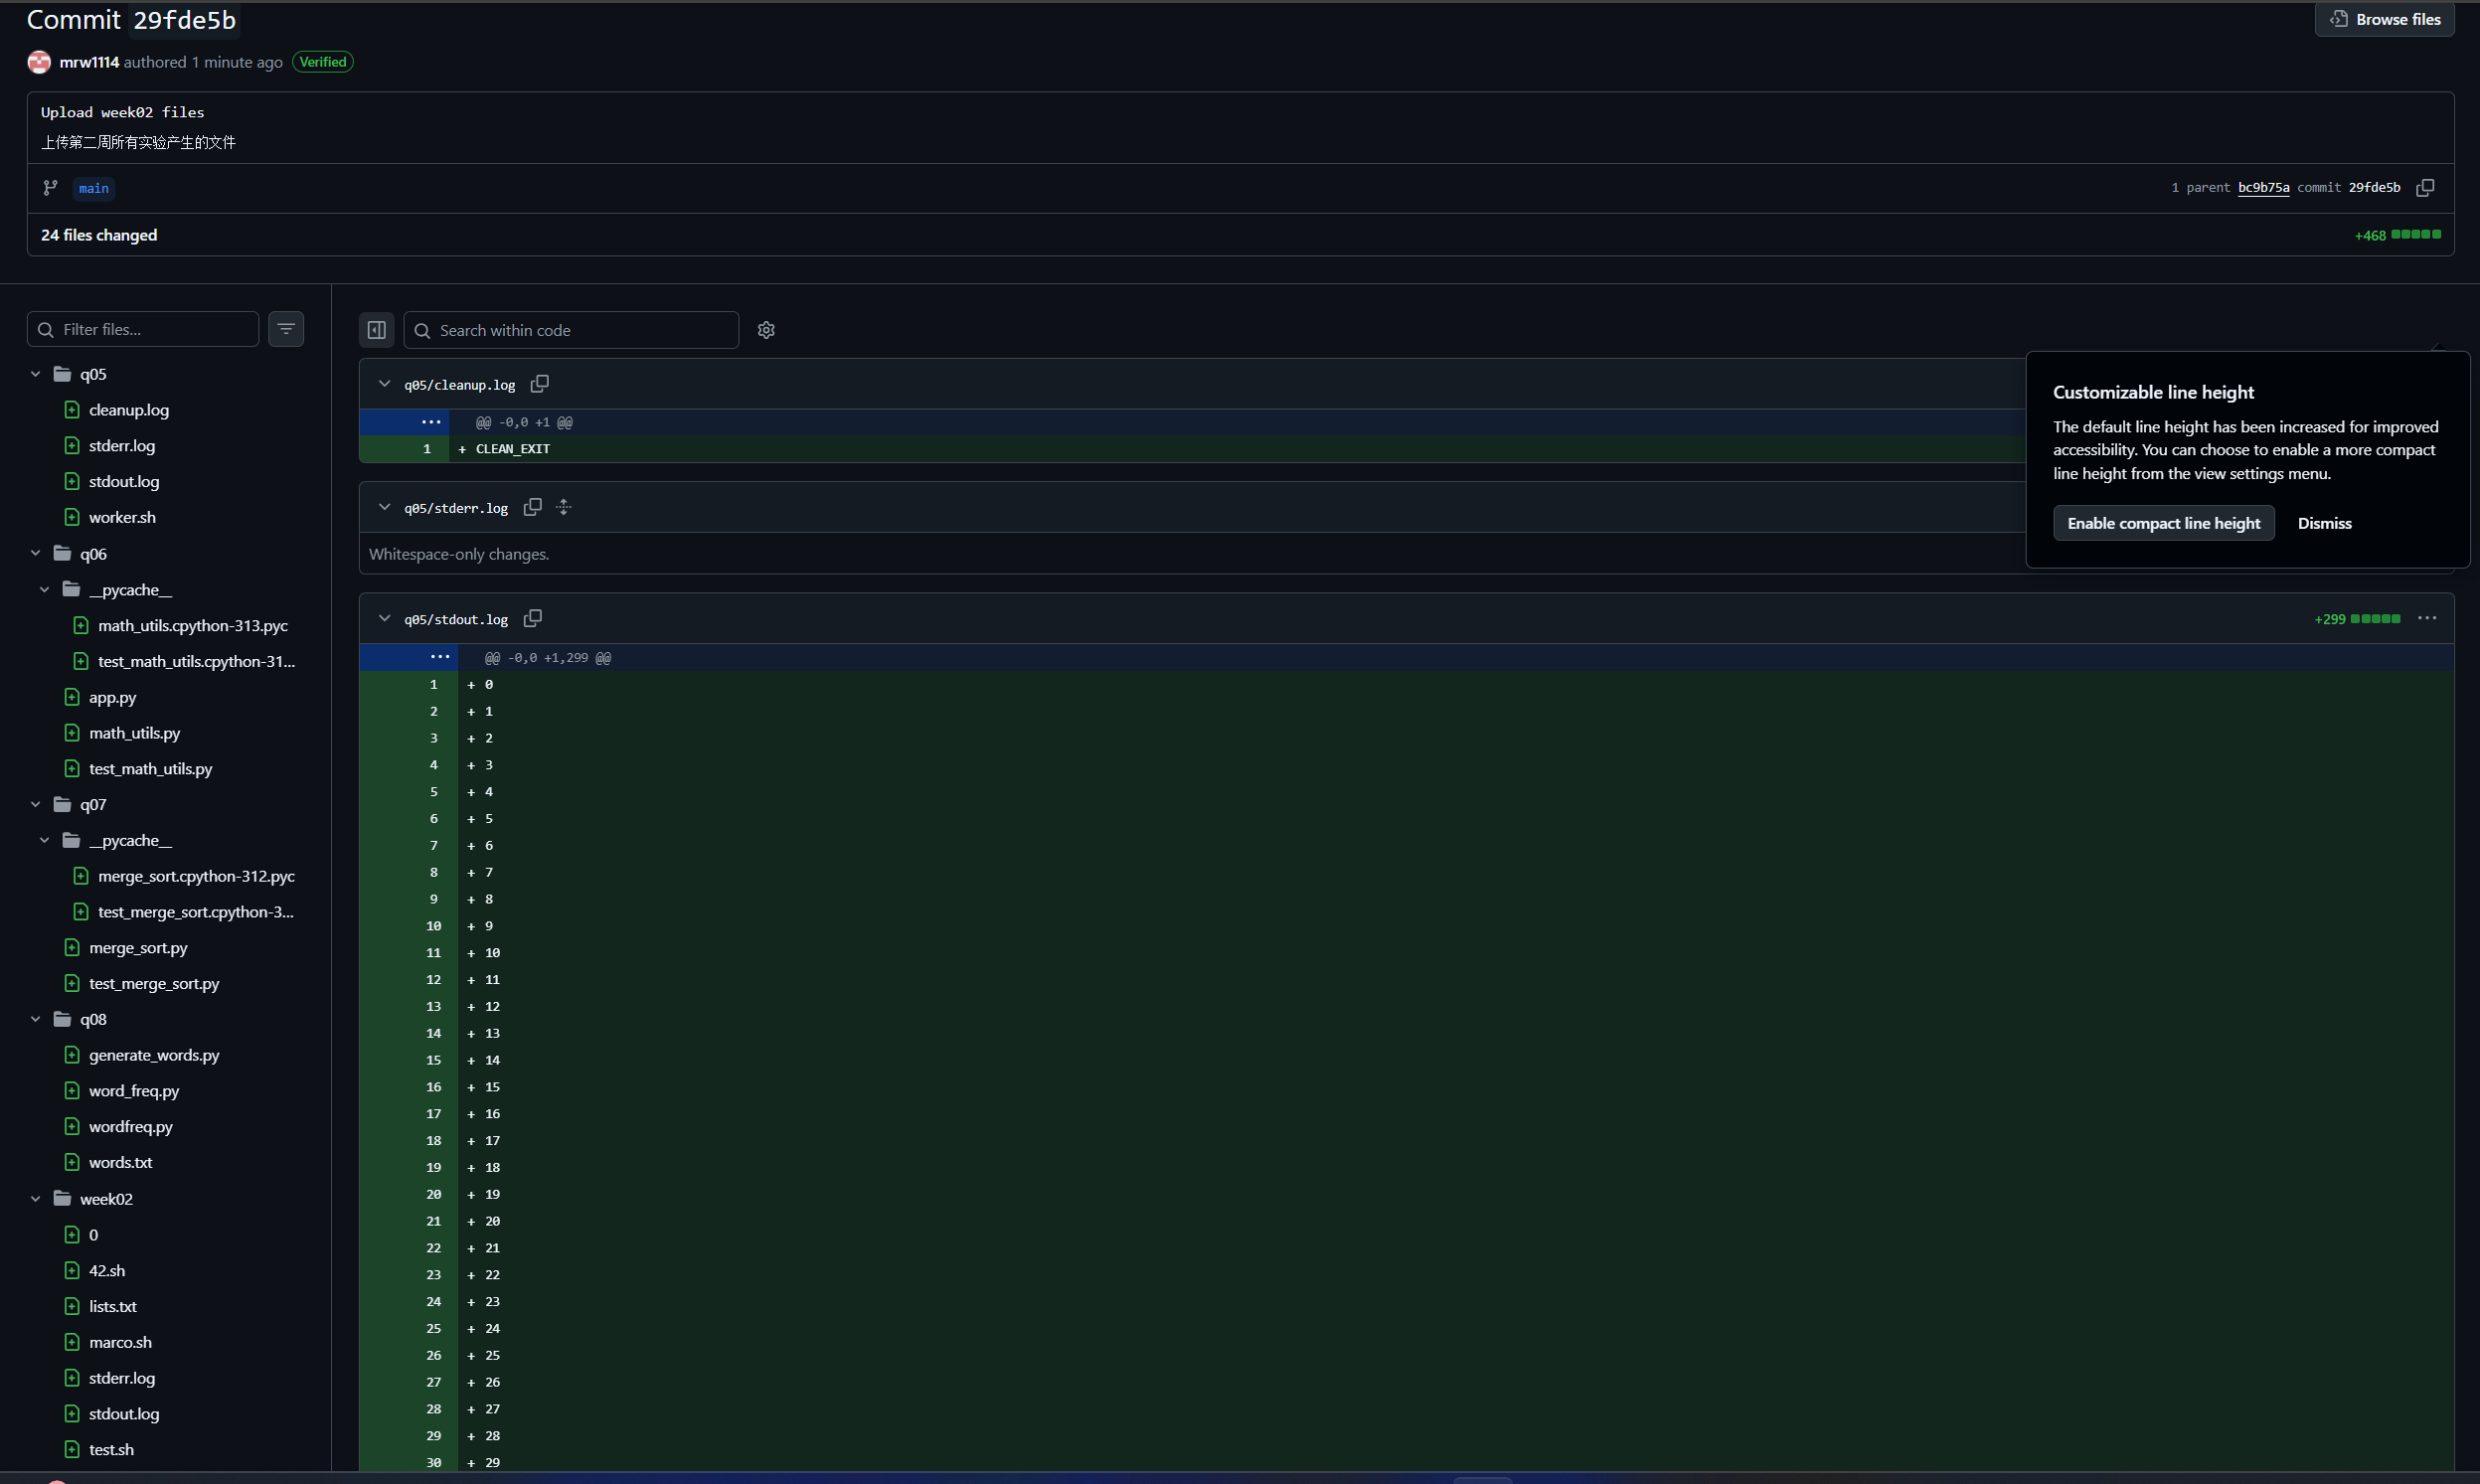
\includegraphics[width=\textwidth]{history2.png}
    \caption{第二周实验提交记录}
    \label{history2}
  \end{figure} 
\end{document}
